\chapter{ローカルデータベースのチュートリアルと普及状況} \label{cap:appA}

\section{チュートリアルと普及状況}
ローカルデータベースの機能の普及を目的として、2020年2月にCERN研究所にてシステムのチュートリアルを行った。
このチュートリアルは以下のような2つのセッションに分けて行った。

\begin{itemize}
  \item 参加者が実際にサーバーの設定、各ソフトウェアのインストールを行いながら機能を実践するセッション(2月3日から6日まで)
  \item 私が参加者の前で実際に機能を実践し、システムや使い方に対して議論を行うセッション(2月7日)
\end{itemize}

それぞれのセッションの様子を図\ref{Tutorial_picture}に示す。
数多くの議論を行い、有益なフィードバックを得ることができた。
また品質試験の流れにおいて、一連の機能確認をすることができた。

\begin{figure}[bpt]
  \begin{center}
  \begin{minipage}{0.4\hsize}
    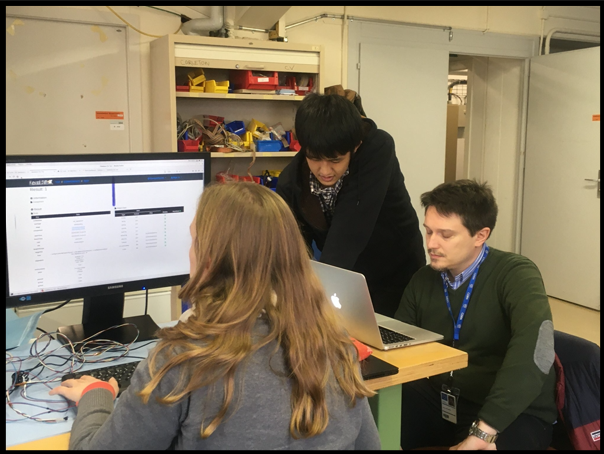
\includegraphics[width=6cm]{hands_on}
  \end{minipage}
  \begin{minipage}{0.4\hsize}
    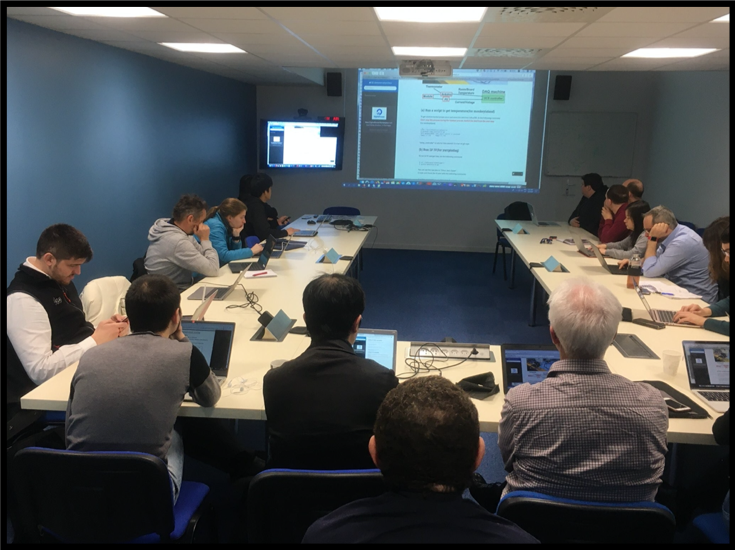
\includegraphics[width=6cm]{hands_off}
  \end{minipage}
  \caption[ローカルデータベースシステムチュートリアルの様子]{ローカルデータベースシステムチュートリアルの様子。2020年2月にCERNでローカルデータベースシステムのチュートリアルを行った。参加者が実際にシステムの設置、機能実行を行うハンズオンセッション(左図)と、参加者の前で実際に機能の動作をみせ、議論を行うハンズオフセッション(右図)に分けて行った。システムに有益な情報を獲得したと共に、システムの機能普及に成功した。}
  \label{Tutorial_picture}
  \end{center}
\end{figure}

これを経て現在ローカルデータベースは世界18箇所にて導入され、試験運用が開始している。
将来的には全組み立て機関で使うことが決定しており、それに向けたシステム開発、サポートが必要となっている状況である。
ローカルデータベースについて、導入及び試験運用を行っている機関を以下に示す。また世界地図を\ref{localdb_world_map}に示す。

\begin{itemize}
  \item 高エネルギー加速器研究機構(KEK), 日本
  \item 欧州原子核研究機構(CERN), スイス
  \item University of Liverpool, イギリス
  \item University of Oxford, イギリス
  \item University of Glasgow, イギリス
  \item Paris-Saclay University, フランス
  \item パリ第6大学, フランス
  \item フランス国立科学研究センター, フランス
  \item University of Grenoble, フランス
  \item University of Gottingen, ドイツ
  \item University of Siegen, ドイツ
  \item University of Genoa, イタリア
  \item University of Salento, イタリア
  \item University of Milan, イタリア
  \item University of Udine, イタリア
  \item Univerity of Trento, イタリア
  \item University of Oklahoma, アメリカ
  \item Argonne National Laboratory, アメリカ
  \item Lawrence Berkeley National Laboratory(LBL), アメリカ
\end{itemize}

\begin{figure}[bpt]\centering
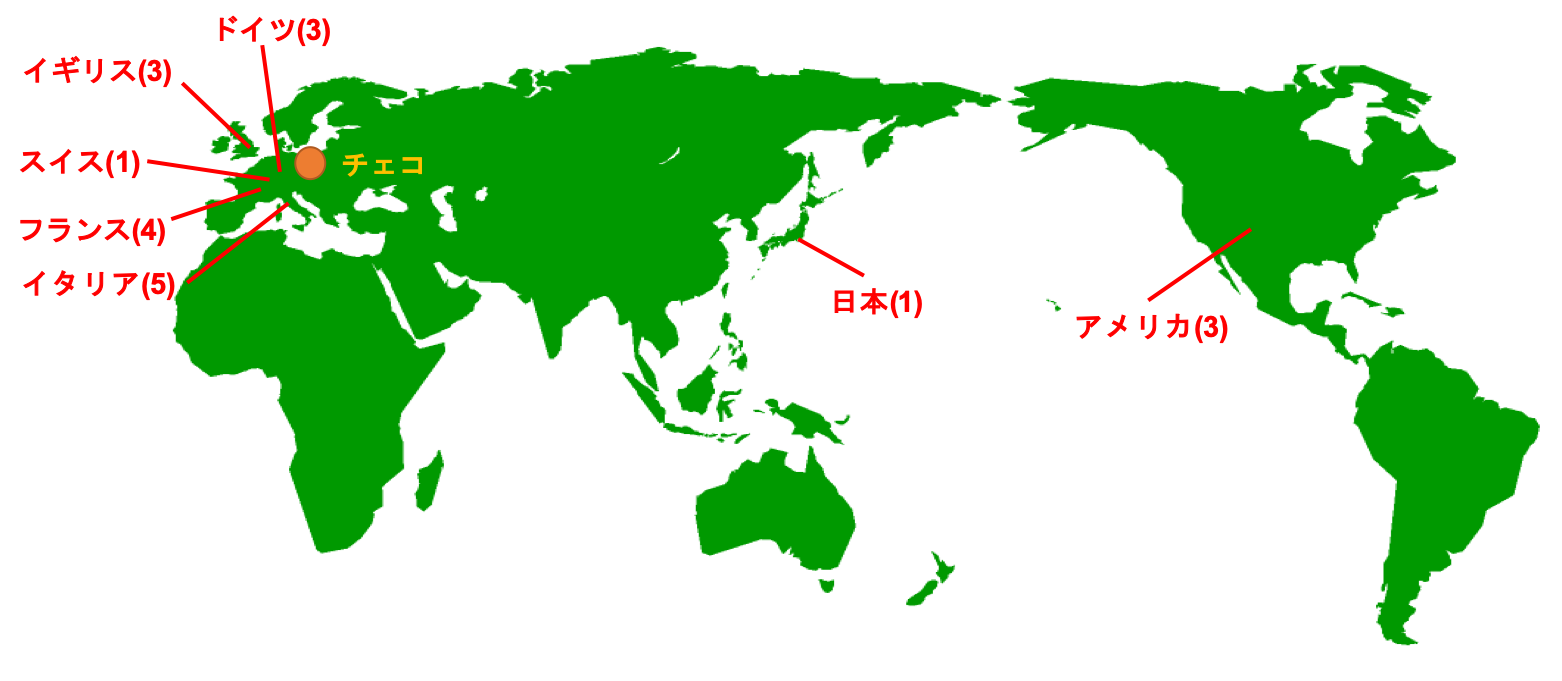
\includegraphics[width=14cm]{localdb_world_map}
\caption[ローカルデータベースシステム導入及び試運転場所]{ローカルデータベースシステム導入及び試運転場所。赤文字は設置している地域、括弧内の数字はその地域におけるシステム導入場所の数を示している。2020年11月現在、ローカルデータベースシステムは世界18の機関で試験運転がなされている。日本を除いてその多くはヨーロッパとアメリカに位置していることが分かる。}
\label{localdb_world_map}
\end{figure}


